\section{Admin Usage}
\label{sec:admin_usage}
The use cases \tucadmin[] and \gstat[], which are described in section \ref{sec:usecase}, are the two main usages of the application which the \admin[] will use.
The \tucadmin[] use case is divided into two usages; manage people and manage departments.
These three usages are described in subsections \ref{sub:managePeople}, \ref{sub:managedep}, and \ref{sub:statisticsadmin}.

\subsection{Manage People}
\label{sub:managePeople}
For an \admin[] to manage the people in the application -- or rather the people's users -- he/she can click the menu point called Manage People which can be seen in figure \ref{fig:master}.
The view which the \admin[] is presented with is a table of all the users in the application.
The table includes: Actions on the user, id number, e-mail, department name, workload, and the roles of the user.
The department name and workload is only available for \astaff[] users, because they are the only ones with a department and a workload.
Other users simply gets ``N/A'' in these cells of the table.
The actions on the users are: Edit, delete, reset password.
This is done by clicking the corresponding link next to the user which the action is to be invoked on.

The edit link takes the \admin[] to the edit view of the corresponding user.
From here he/she can see the id and user name of the user, and can edit the e-mail, department, and the roles of the user.
The department can only be edited if the user is a staff member.
If a non-\astaff[] user is given the \astaff[] role, the \admin[] is asked to give the user a department, because we do not want to \astaff[] members without a department.

The deletion of a user will result in permanent removal of the user from the application.
This can only happen if the user is not subscribed to any problems and is not assigned to any problems.

The reset password action initiates a random password generator to set as the new password for the given user.
After that an e-mail is sent to the user containing the newly generated password.

\subsection{Manage Departments}
\label{sub:managedep}
The menu point Manage Departments which is seen in figure \ref{fig:master} allows the \admin[]s to administrate the departments, categories, and tags in the application.
The view shown when this menu point is clicked, the \admin[] is presented with a list of every department in the application along with a link to create a new department.

When creating a new department, the \admin[] creating it must provide the name of the department and a description.
A newly created department is initially empty, i.e. it contains no categories and no \astaff[] members are part of it.
To add categories and \astaff[] members an \admin[] can select the department in the list of the Manage Department view.

\begin{figure}[htb]
	\centering
		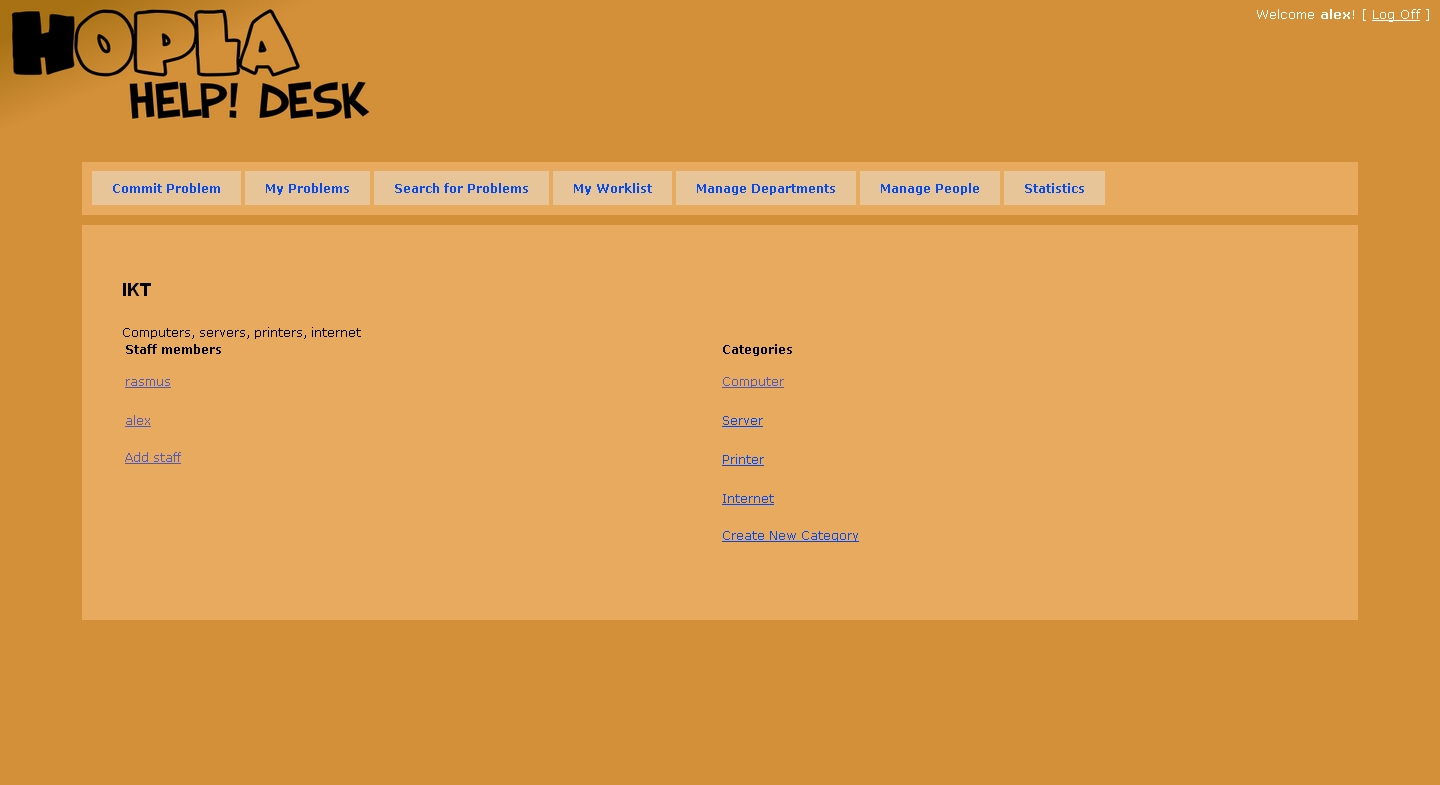
\includegraphics[width=1.00\textwidth, clip=true, trim=2.9cm 6cm 10cm 8cm]{input/implementation/program_presentation/department.png}
	\morscaption{The department view, note that the screen shot has been cropped}
	\label{fig:department}
\end{figure}

When a department is selected, the \admin[] is presented with a view similar to figure \ref{fig:department}.
The view contains two lists; one with the \astaff[] members associated with the department and one with the categories associated with the department.
Links to add a new category and to attach \astaff[] member to the department are also provided in this view.
These two parts of the department view are described in the following sub-subsections.

\subsubsection{Manage \astaff[c] Members}
When a \astaff[] member is selected, the \admin[] is redirected to the person editor of that \astaff[] member, which is described in subsection \ref{sub:managePeople}.
To add a \astaff[] member to the selected department, the \admin[] can click the Add staff link in the department view.
This renders a view with a table of every person in the application who has the \astaff[] role.
The table resembles the table described in subsection \ref{sub:managePeople} except that the id for the \astaff[] members are not shown.

\subsubsection{Manage Categories}
To create a category, an \admin[] clicks on the corresponding link and provides a name and description for the category.
Like a newly created department, the new category is empty, thus containing no tags.
To change the new category -- or another one -- an \admin[] can click on it in the department view for the department which the category belongs to.
The view which is then presented shows the id, name, description, department, and whether or not the category is hidden.
Furthermore the category can be deleted, hidden, and edited from this view.
Hiding a category will hide all the tags associated to that category.
If the category is hidden it can be unhidden(revealed), which will unhide all the tags associated to the category.
To delete a category, every tag must be removed beforehand.
It is possible to create new tags from the category view, these tags will initially be attach to the category from which they were created.

During creation of a tag, the \admin[] must provide a name for tag, a description, and a priority.
The priority of a tag is a number which indicates how important a problem with the tag is relatively to problems with other tags.
There is no inbuilt scale, if the organization using out application wants their tags to vary in priority from 0 to 10 they can do that, the only constraint is that the priority is a 16 bit integer, resulting in a range from $2^{15}$ to $2^{15}-1$.

In the category view, the tags can also be individually be hidden, edited, viewed in details, and deleted.
Hiding a tag means that it will not be shown in e.g. the problem search view of the \aclient[]s.
When editing a tag, the \admin[] can set the same properties of the tag as when a tag is created.
The detailed view of a tag shows the properties of the given tag, namely: Id, name, description, priority, category id, number of solved problems, time consumed, average time spend, and whether or not it is hidden.
The time consumed indicates the time, in minutes, for how long every problem with this tag has taken to solve.
It is used along with number of problems solved to calculate the average time spend to solve problems with that tag.
This is again used to calculate the estimated time of completion of unsolved problems.

To delete a tag, no problem can be associated with it.
The deletion of tags is only supposed to be used if a tag is created incorrectly, e.g. another tag already exists or it is created in the wrong department.

\subsection{\gstat[c]}
\label{sub:statisticsadmin}
\begin{figure}[htb]
	\centering
		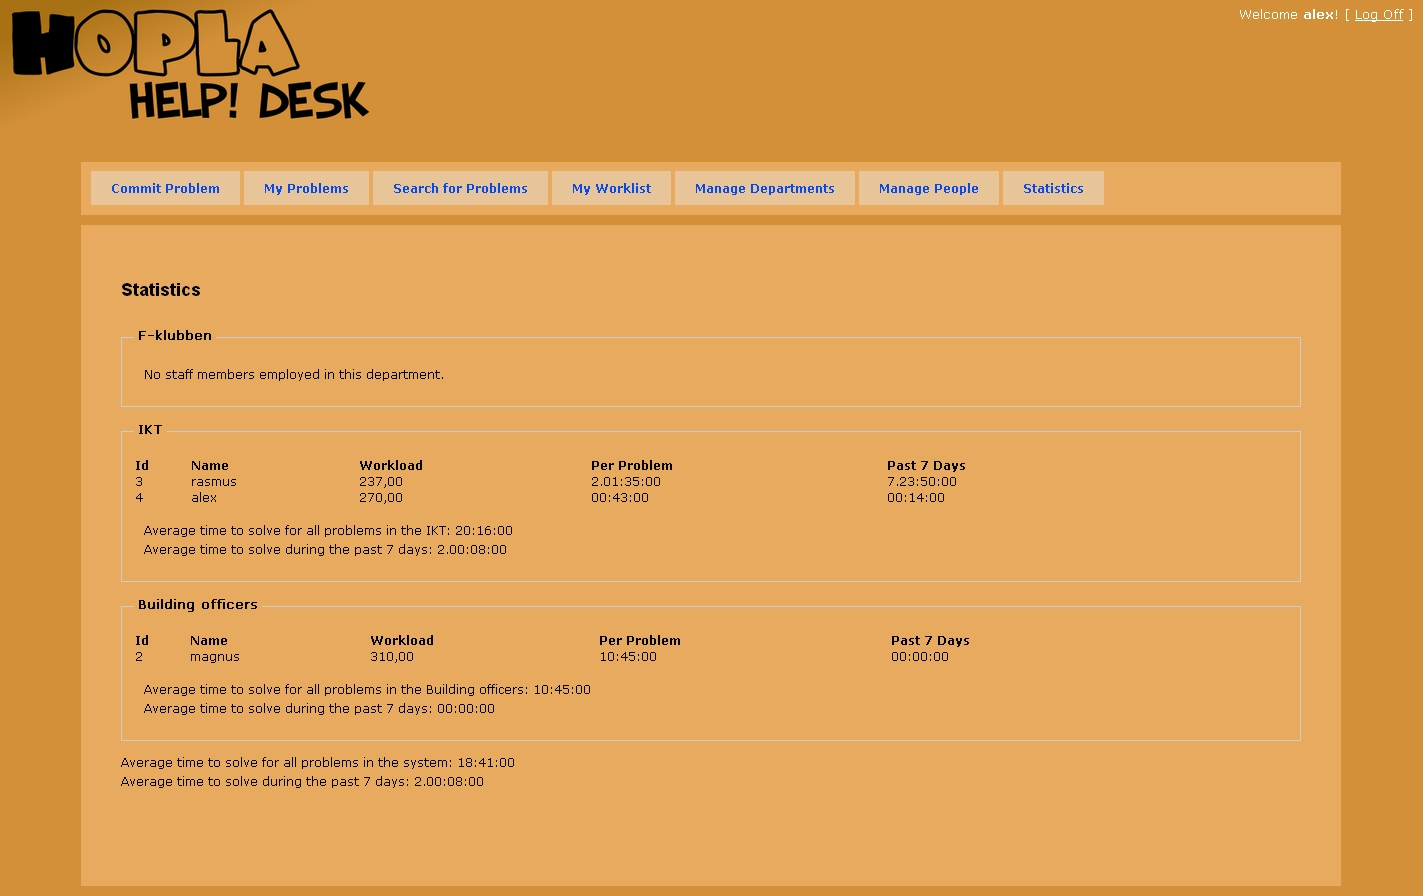
\includegraphics[width=1.00\textwidth, clip=true, trim=2.9cm 2.5cm 15cm 8cm]{input/implementation/program_presentation/stat.png}
	\morscaption{The statistics view, note that the screen shot has been cropped}
	\label{fig:stat}
\end{figure}
An \admin[] can get statistics about how long problems in average remain unsolved.
To do this he/she must select the Statics menu point as seen in figure \ref{fig:master}.
He/she is then presented with a view which shows the average time for a problem to remain unsolved for each particular \astaff[] member, each department, and for the application over all.
It also shows the average time for problems to be solved for the last week for all of the three groups above.
This is seen in figure \ref{fig:stat}.

These statistics can be used in any way the \admin[] wants, e.g. to see if a particular department needs more \astaff[] members if that given department is generally slower than the others.
It is only \admin s who are allowed to see this page because \aclient s might use the statistics to categorize their problem, so that it will end up in the department which is generally fastest to solve problems, but this will actually make the problem be solved slower if the \astaff[] member has to figure out where to reassign it.
The \astaff[] members can neither see this page in order to avoid internal competition for fastest solve time, because it could lead to a lack in quality of the solutions.

%%The last thing might be removed, I am not sure whether it is too much or allrigth.

